%*----------- SLIDE -------------------------------------------------------------
\begin{frame}[t]{Lei de Moore}
    %\framesubtitle{Lei de Bradford}
    % \begin{figure}
    %     %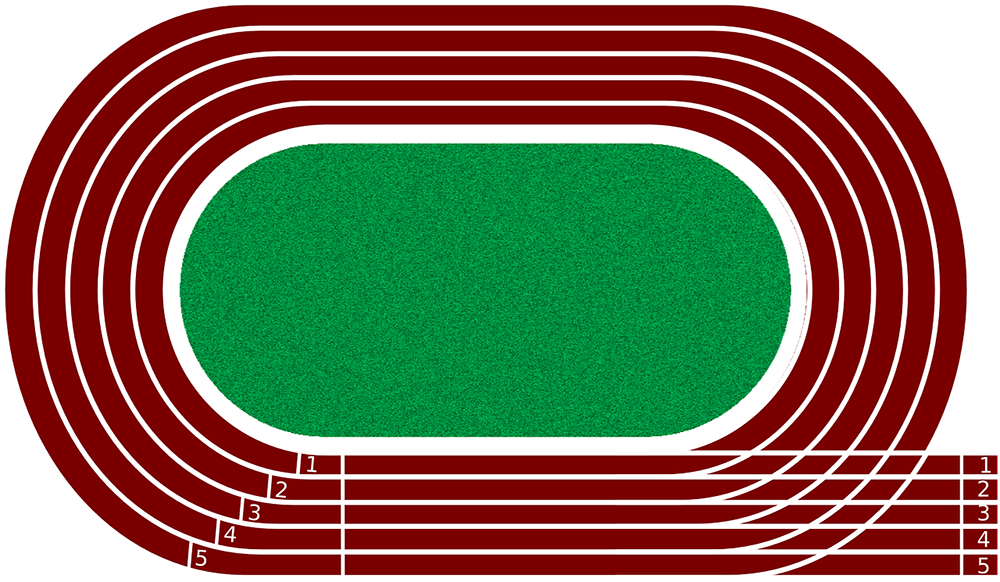
\includegraphics[width=0.7\textwidth]{pista_corrida}
       
    %     \roundpic[xshift=0cm,yshift=0cm]{3cm}{7cm}{pista_corrida}
          
    %     \caption{Formato de um pista de corrida.\cite{agostini2007}}
    % \end{figure}
        \begin{columns}
            \column{.5\textwidth}
                \begin{figure}
                    \roundpic[xshift=1cm,yshift=0cm]{5.8cm}{9cm}{moore.jpeg}
                 %\caption{.}
                \end{figure}
            \column{.48\textwidth}
            \LARGE
            "A densidade de transistores em um chip dobra a cada 18 meses mantendo o mesmo custo de fabricação."\\
            Gordon E. Moore, 1965
            \column{.02\textwidth}
        \end{columns}
        %\column{.01\textwidth}
%*----------- notes
    \note[item]{Notes can help you to remember important information. Turn on the notes option.}
\end{frame}
% %*----------- SLIDE -------------------------------------------------------------
\begin{frame}[t]{Lei de Moore}
    \begin{columns}
        \column{.6\textwidth}
        \begin{figure}
            \centering
            \textbf{Evolução dos Microprocessadores}\par\medskip
            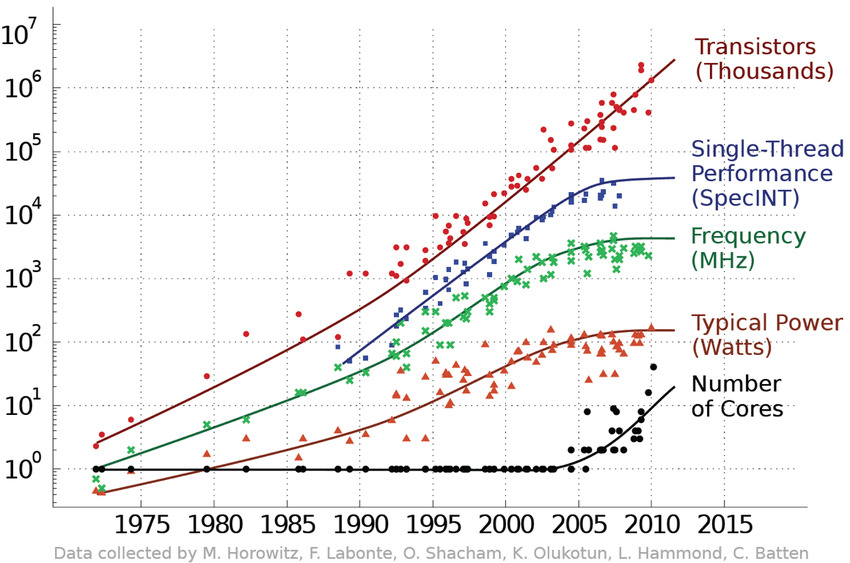
\includegraphics[trim = 0 20 0 0, clip, width=1
            \textwidth]{trends.jpg}
            %\caption{.}
        \end{figure}
        \column{.4\textwidth}
        \itemize
        \item O número de transistores por chip cresceu em escala logarítimica
        \item O aumento no número de transistores parou de refletir no aumento da performance
        \item O consumo energético se tornou muito alto
    \end{columns}
    
        %\column{.01\textwidth}
%*----------- notes
    \note[item]{Notes can help you to remember important information. Turn on the notes option.}
\end{frame}
% %*----------- SLIDE -------------------------------------------------------------
\begin{frame}[t]{Programação em paralelo}
    \framesubtitle{Porquê usar GPUs?}
    \begin{columns}
        \column{.7\textwidth}
        \begin{figure}
            \centering
            \textbf{Performance das GPUs vs CPUs em GFLOPS/s}\par\medskip
            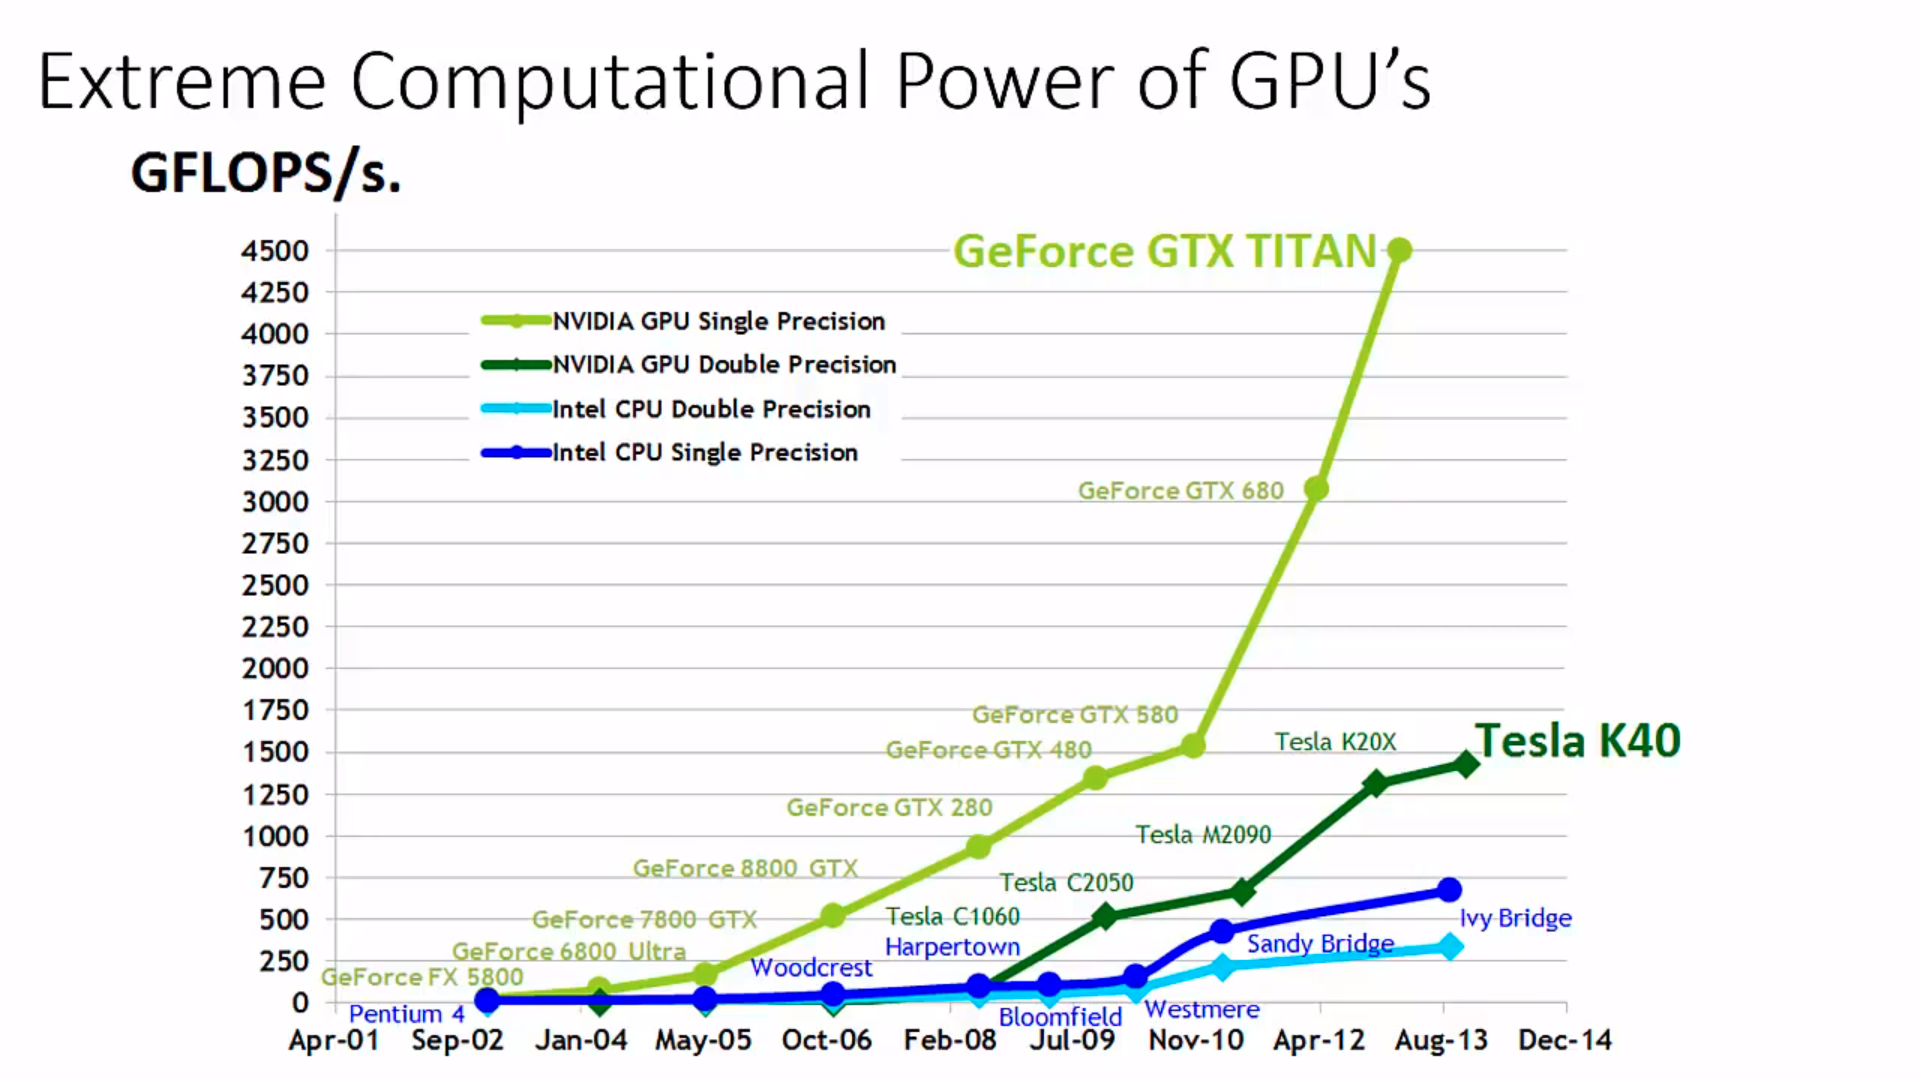
\includegraphics[trim = 80 0 150 130, clip, width=.9
            \textwidth]{gpuvccpu.png}
        \end{figure}
        \column{.3\textwidth}
        \itemize
        \item Poder computacional muito superior das GPUs
        \item Reduzir o tempo de solução de um problema
        \item Resolver problemas mais complexos
    \end{columns}
        
        %\column{.01\textwidth}
%*----------- notes
    \note[item]{Notes can help you to remember important information. Turn on the notes option.}
\end{frame}
% %*----------- SLIDE -------------------------------------------------------------
\begin{frame}[t]{O que é CUDA?}
    \begin{columns}
        \column{.02\textwidth}
        \column{.48\textwidth}
            % \vspace{.4cm}
            \Large
            \begin{itemize}
                \item É um modelo de programação em paralelo que permite o uso da GPU
                \item É basicamente C/C++ com algumas extensões
                \item Pode ser usado em outras linguagens como Fortran e Python 
            \end{itemize}
        \column{.48\textwidth}
            \begin{figure}
                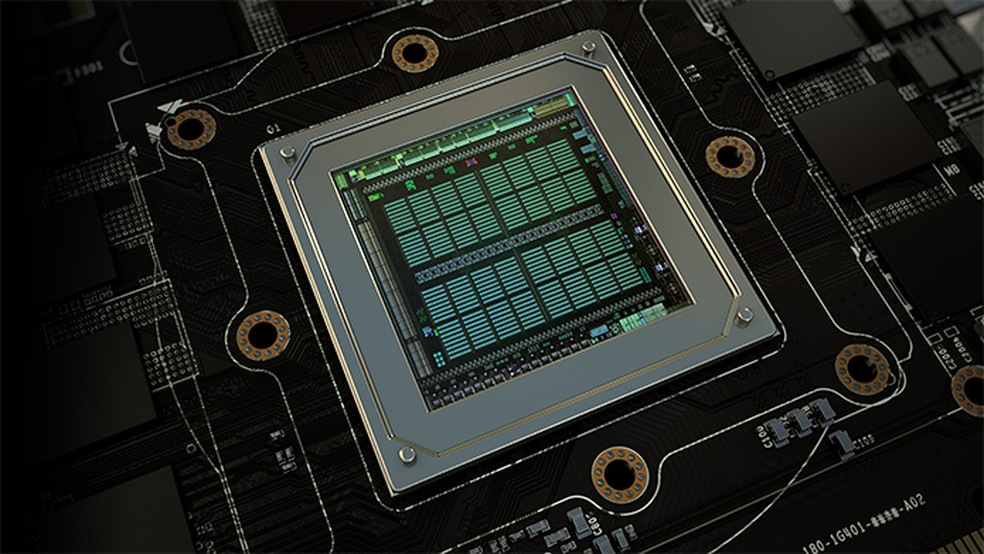
\includegraphics[trim = 180 0 150 0, clip, width=.8
                \textwidth]{2017-04-12-nvidia-gpu.jpeg}
                %\caption{.}
            \end{figure}  
        \column{.02\textwidth}      
    \end{columns}
        %\column{.01\textwidth}
%*----------- notes
    \note[item]{Notes can help you to remember important information. Turn on the notes option.}
\end{frame}
% %*----------- SLIDE -------------------------------------------------------------
\begin{frame}[t]{Aplicações}
    \begin{columns}
        \column{.02\textwidth}
        \column{.48\textwidth}
            % \vspace{.4cm}
            \Large
            \begin{itemize}
                \item Processamento de imagens
                \item Simulações
                \item Cálculos vetoriais e matriciais
                \item Algoritimos de buscas
                \item Química computacional
                \item Ordenação
                \item Inteligência computacional
                \item Deep learning
            \end{itemize}
        \column{.48\textwidth}
            \begin{figure}
                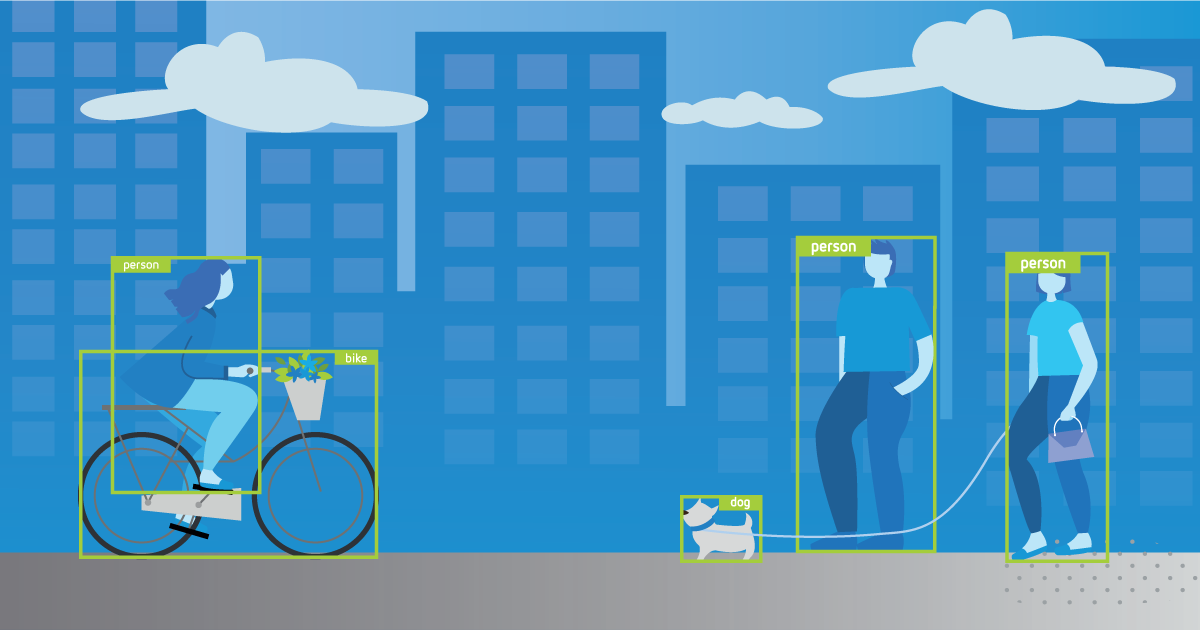
\includegraphics[trim = 600 0 0 0, clip, width=.85
                \textwidth]{object-detection-illustration.png}
                %\caption{.}
            \end{figure}  
        \column{.02\textwidth}      
    \end{columns}
        %\column{.01\textwidth}
%*----------- notes
    \note[item]{Notes can help you to remember important information. Turn on the notes option.}
\end{frame}


% %-
% %*----------- SLIDE -------------------------------------------------------------
% \begin{frame}[t]{As principais leis bibliométricas}
%     \framesubtitle{Lei de Bradford}
%     % \begin{figure}
%     %     %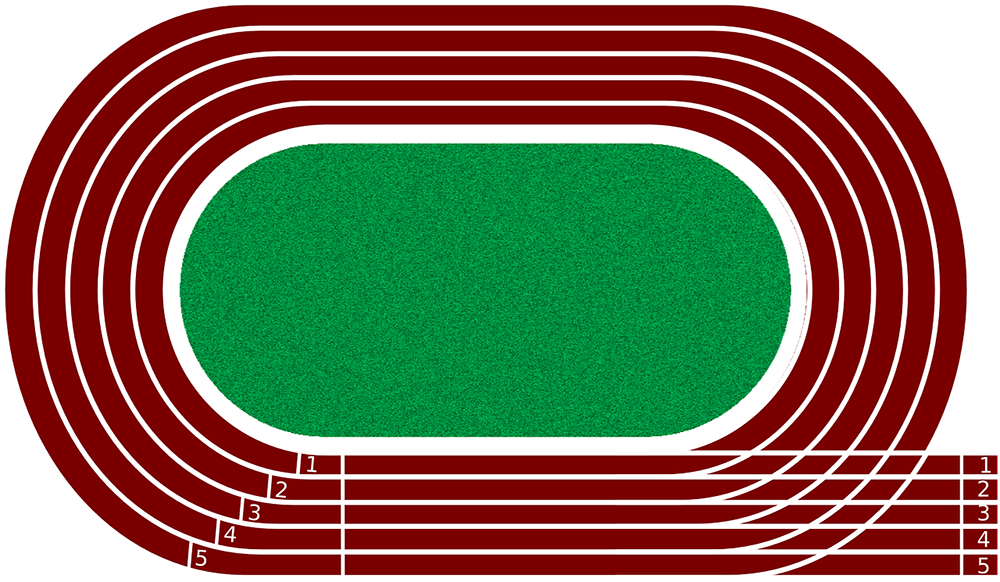
\includegraphics[width=0.7\textwidth]{pista_corrida}
       
%     %     \roundpic[xshift=0cm,yshift=0cm]{3cm}{7cm}{pista_corrida}
          
%     %     \caption{Formato de um pista de corrida.\cite{agostini2007}}
%     % \end{figure}

%     \begin{columns}
%         \column{.1\textwidth}
%         \column{.3\textwidth}

%         \begin{figure}
%             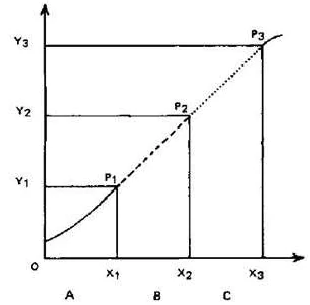
\includegraphics[trim = 0 0 0 0, clip, width=0.7\textwidth]{bradford-2.png}
%             %\caption{.}
%         \end{figure}

%         \centering
%         $F(x) = a + b \log x$
%         \column{.69\textwidth}
%         A lei de Bradford objetiva conhecer o núcleo de periódicos produzidos em determinado tema.\\
%         \scriptsize{
%             Bradford realiza uma série de estudos que culminam, em 1934, com a formulação da \textbf{lei da dispersão}.\\
%             O autor percebe que, numa coleção de periódicos sobre geofísica, existe sempre um núcleo menor de periódicos relacionados de maneira estreita, sendo que o número de perióidocs em cad zona aumenta, enquanto a produtividade diminui.\\
%             Analisando 326 períodicos, ele descobriu que 9 periódicos continham 429 artigos, 59 continham 499 e 258 continham 404 artigos.
%         }
%     \end{columns}

%     \vspace*{0.2cm}
%     \begin{itemize}
%         \item Medir produtividade dos periódicos
%         \item Estabelecer núcleo e as áreas de dispersão 
%         \item Permite fazer a estimativa do grau de relevância das revistas de conhecimentos
%     \end{itemize}
% %*----------- notes
%     \note[item]{Notes can help you to remember important information. Turn on the notes option.}
% \end{frame}
%-
%*----------- SLIDE -------------------------------------------------------------
\begin{frame}[t]{GPU x CPU}
    \framesubtitle{Qual a diferença?}
    \begin{figure}
        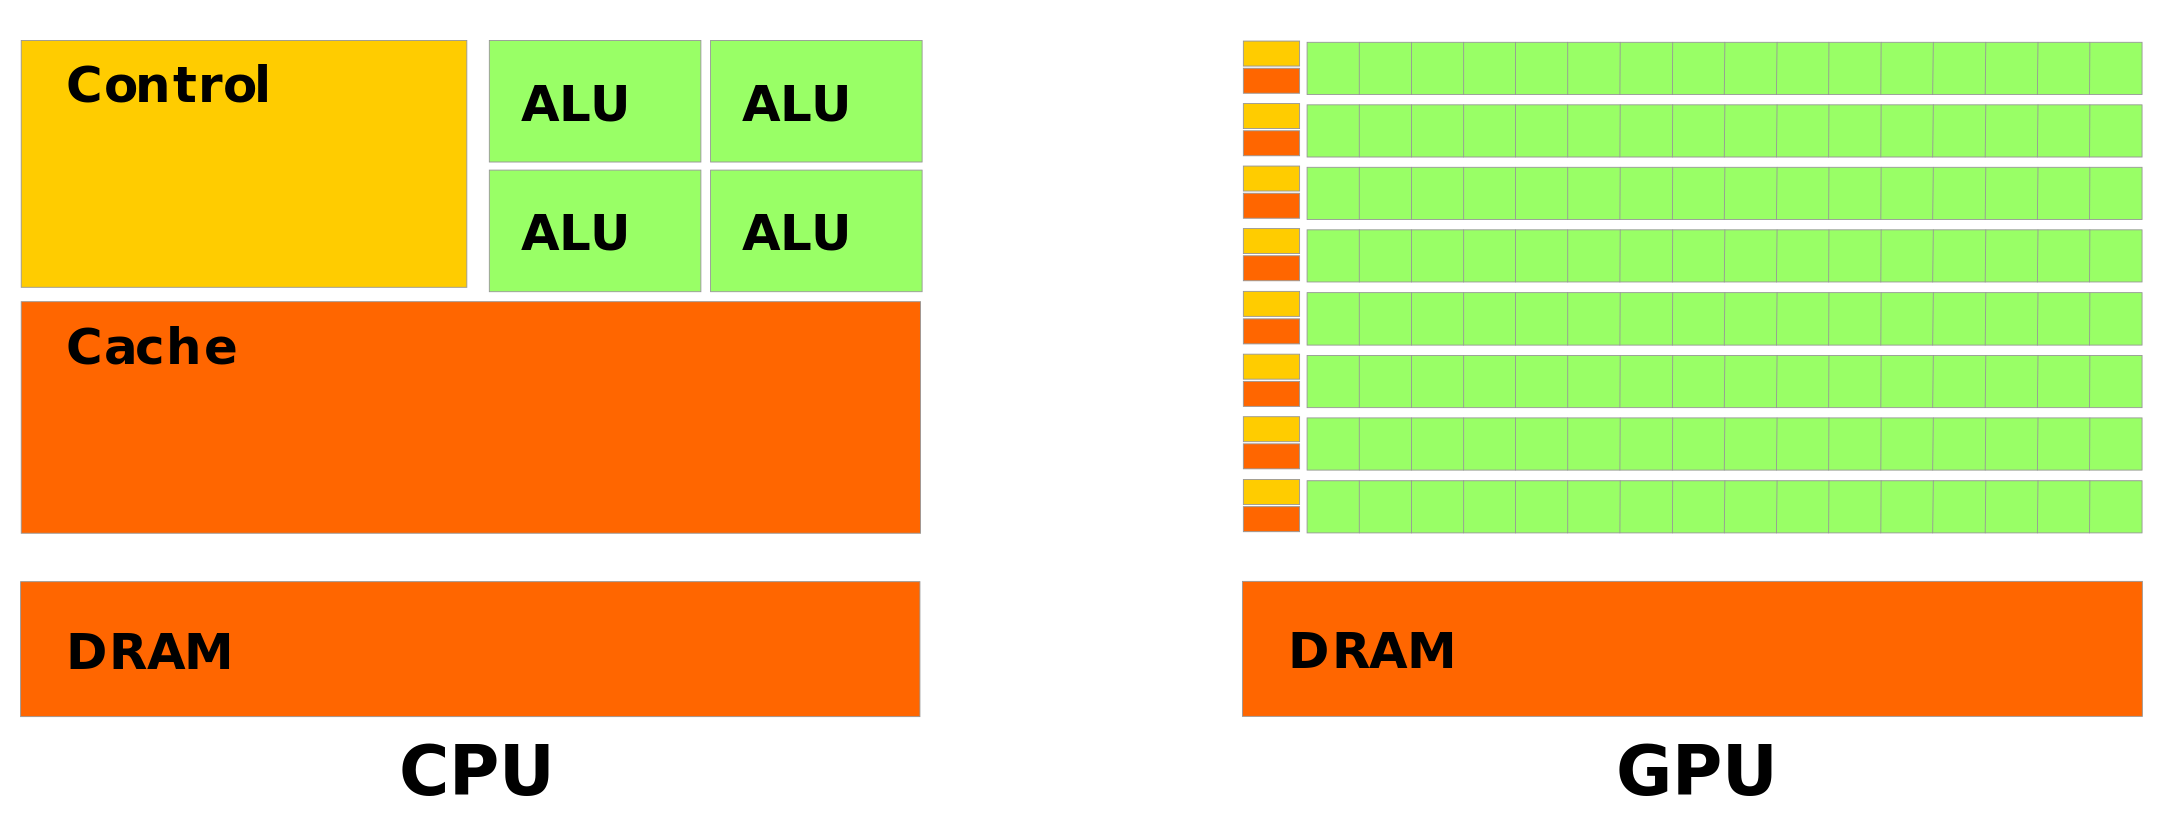
\includegraphics[trim = 0 0 0 0, clip, width=1\textwidth]{Cpu-gpu.png}
        %\caption{.}
    \end{figure}

%*----------- notes
    \note[item]{Notes can help you to remember important information. Turn on the notes option.}
\end{frame}
%*----------- SLIDE -------------------------------------------------------------
\begin{frame}[t]{Nvidia G80}
    \framesubtitle{GeForce 8800}
    \begin{figure}
        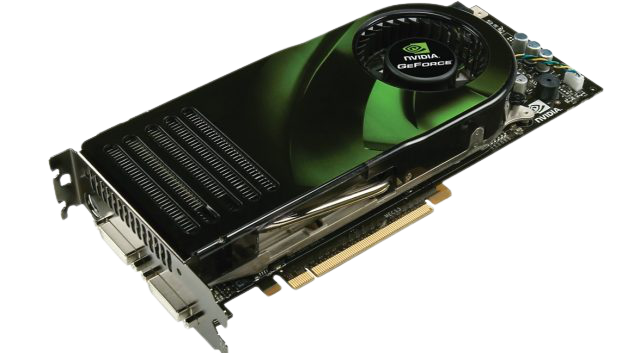
\includegraphics[trim = 0 0 0 0, clip, width=0.7\textwidth]{g80.png}
        %\caption{.}
    \end{figure}

%*----------- notes
    \note[item]{Notes can help you to remember important information. Turn on the notes option.}
\end{frame}
%-
%*----------- SLIDE -------------------------------------------------------------
\begin{frame}[t]{Arquitetura CUDA}
    % \framesubtitle{Lei de Zipf}
    \begin{figure}
        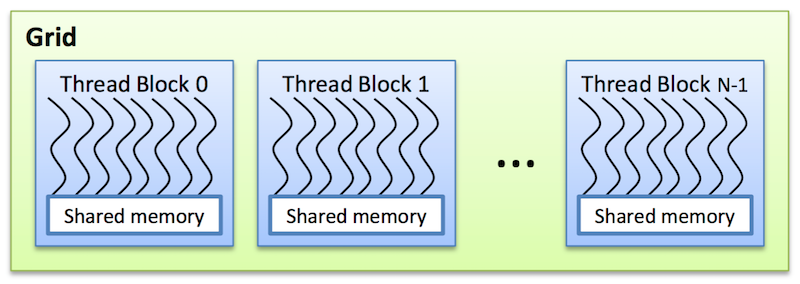
\includegraphics[trim = 0 0 0 0, clip, width=0.7\textwidth]{02-threadgrid.png}
    \end{figure}
    \begin{columns}
        \column{.15\textwidth}
        \column{.35\textwidth}
            \begin{figure}
               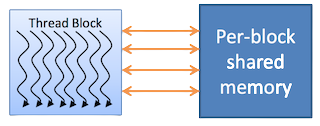
\includegraphics[trim = 0 0 0 0, clip, width=1\textwidth]{02-sharedmemory-removebg-preview.png}
            \end{figure}
        
        \column{.35\textwidth}
            \begin{figure}
               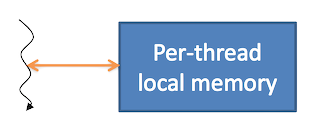
\includegraphics[trim = 0 0 0 0, clip, width=1\textwidth]{02-localmemory-removebg-preview.png}
            \end{figure}
        \column{.15\textwidth}    
    \end{columns}
%*----------- notes
    \note[item]{Notes can help you to remember important information. Turn on the notes option.}
\end{frame}
%-
\begin{frame}[t]{Arquitetura CUDA}
    % \framesubtitle{Qual a diferença?}
    \begin{figure}
        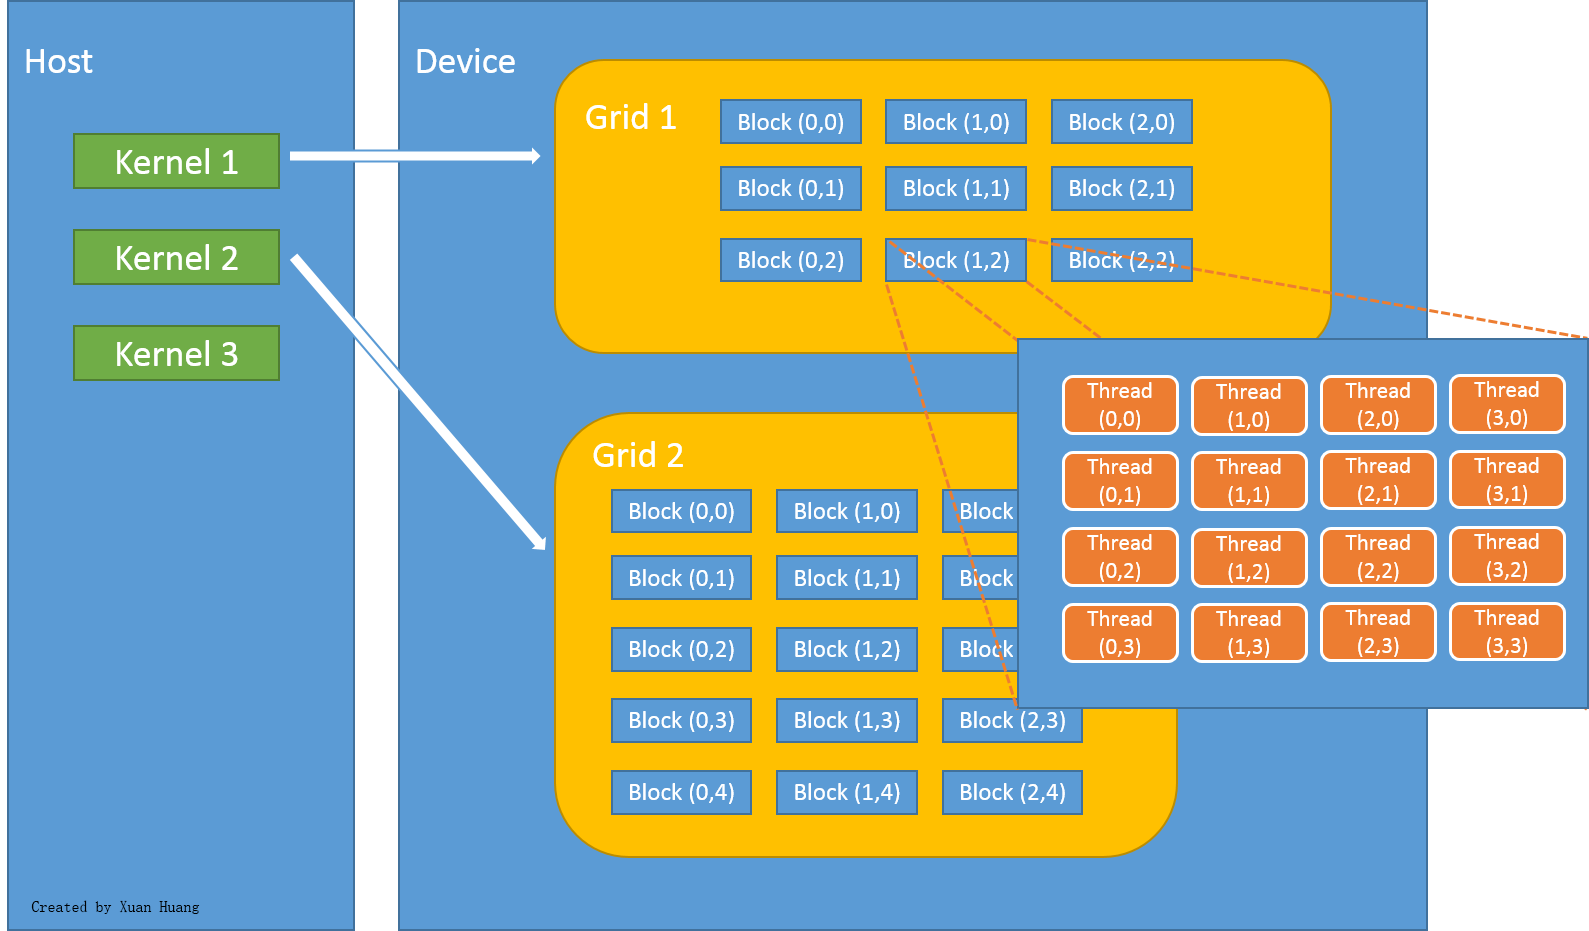
\includegraphics[trim = 0 0 0 0, clip, width=0.78\textwidth]{threadblock.png}
        %\caption{.}
    \end{figure}

%*----------- notes
    \note[item]{Notes can help you to remember important information. Turn on the notes option.}
\end{frame}
% %*----------- SLIDE -------------------------------------------------------------
\begin{frame}[t]{Modelo de Memória}
    % \framesubtitle{Qual a diferença?}
    \begin{columns}
        \column{0.5\textwidth}
            \begin{figure}
                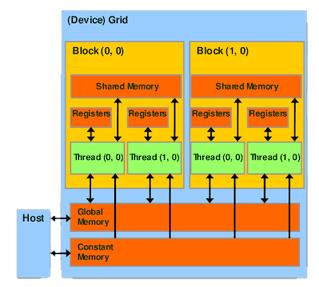
\includegraphics [trim = 0 0 0 0, clip, width=1\textwidth]{MEMORYY.png}
                %\caption{.}
            \end{figure}    
        \column{0.5\textwidth}
        \itemize
        \item O host se comunica com o device através da memória global
        \item Apenas threads de um mesmo Block podem se comunicar e cooperar
        \item Therds de blocks diferentes não se comunicam
        \item Cada thread possui um conjunto de registradores 
    \end{columns}
    % \begin{figure}
    %     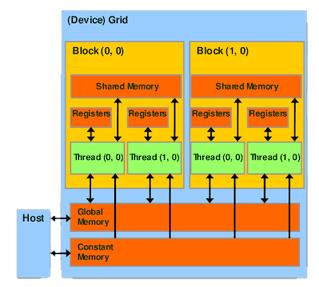
\includegraphics [trim = 0 0 0 0, clip, width=0.5\textwidth]{MEMORYY.png}
    %     %\caption{.}
    % \end{figure}

%*----------- notes
    \note[item]{Notes can help you to remember important information. Turn on the notes option.}
\end{frame}
% %*----------- SLIDE -------------------------------------------------------------
\begin{frame}[t]{Modelo de Memória}
    \framesubtitle{Cooperação em Thread Blocks}
    \begin{columns}
        \column{.05\textwidth}
        \column{.45\textwidth}
            \begin{figure}
               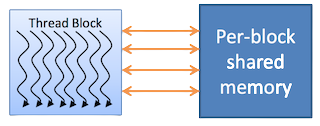
\includegraphics[trim = 0 0 0 0, clip, width=0.9\textwidth]{02-sharedmemory-removebg-preview.png}
            \end{figure}
        
        \column{.5\textwidth}
            \begin{figure}
               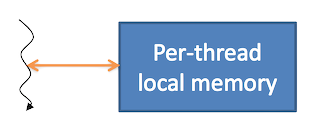
\includegraphics[trim = 0 0 0 0, clip, width=0.9\textwidth]{02-localmemory-removebg-preview.png}
            \end{figure}
        \column{.15\textwidth}    
    \end{columns}
    \vspace*{0.2cm}
    \itemize
    \item Threads podem compartilhar resultados entre si ou cooperar para produzir um resultado único através da memória compartilhada
    \item Threads podem se sincronizar umas com as outras
    \item A memória local é privada para cada thread
    \item A memória compartilhada é mais rápida que a memória global e a local
    % \begin{figure}
    %     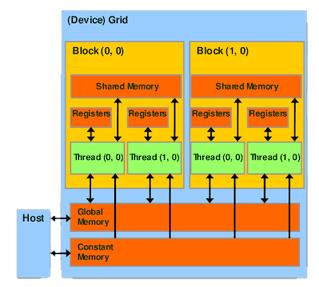
\includegraphics [trim = 0 0 0 0, clip, width=0.5\textwidth]{MEMORYY.png}
    %     %\caption{.}
    % \end{figure}

%*----------- notes
    \note[item]{Notes can help you to remember important information. Turn on the notes option.}
\end{frame}
% %*----------- SLIDE -------------------------------------------------------------
\begin{frame}[t]{Launching do Kernel}
    % \framesubtitle{Cooperação em Thread Blocks}
    \Large{
    \begin{shaded}
        kernel\textless \textless \textless dim3 grid, dim3 block\textgreater \textgreater \textgreater (...)
    \end{shaded}
    }
    \begin{itemize}
    \item O primeiro parâmetro diz quantos blocos você tem no Grid
    \item O segundo parâmetro diz quantas threads tem no Block
    \end{itemize}
    \begin{shaded}
        dim3 grid(16,16);\\
        dim3 block(16,16);\\
        % kernel\textless \textless \textless dim3 grid, dim3 block\textgreater \textgreater \textgreater (...)
    \end{shaded}
    % \begin{figure}
    %     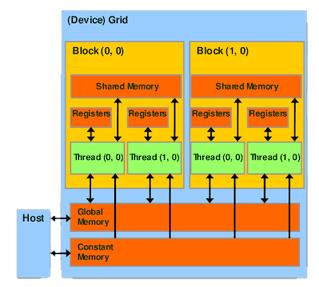
\includegraphics [trim = 0 0 0 0, clip, width=0.5\textwidth]{MEMORYY.png}
    %     %\caption{.}
    % \end{figure}

%*----------- notes
    \note[item]{Notes can help you to remember important information. Turn on the notes option.}
\end{frame}
% %*----------- SLIDE -------------------------------------------------------------
\begin{frame}[t]{Kernel Mínimo}
    % \framesubtitle{Cooperação em Thread Blocks} 
    \Large{
    \begin{shaded}

        \textunderscore \textunderscore  global\textunderscore \textunderscore void mykernel(...)\{\\
        \}
        % \{\\
        % \;\;\;\; int idx = blockDim.x * blockIdx.x + threadIdx.x\\
        % \;\;\;\; a[idx] = 13\\
        % \} \\
    \end{shaded}
    }
    \Large{
    A keyword \textcolor{red}{\textunderscore \textunderscore  global\textunderscore \textunderscore} indica uma função que é executada no device.\\ %e é chamada pelo host.\\
    O compilador nvcc separa o código em componentes de host e componentes de device. Os componentes de device são compilados com o nvcc e os componentes de host por compiladores padrão como gcc.
    }
    
    % \begin{figure}
    %     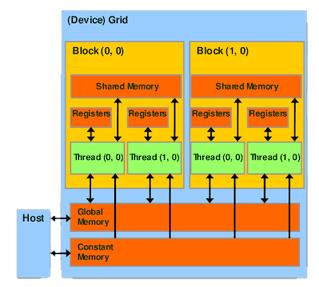
\includegraphics [trim = 0 0 0 0, clip, width=0.5\textwidth]{MEMORYY.png}
    %     %\caption{.}
    % \end{figure}
%*----------- notes
    \note[item]{Notes can help you to remember important information. Turn on the notes option.}
\end{frame}
% %*----------- SLIDE -------------------------------------------------------------
\begin{frame}[t]{Alocação de Memória}
    % \framesubtitle{Cooperação em Thread Blocks} 
    \Large{
    \begin{shaded}
        \itemize
        \item cudaMalloc() $\rightarrow$ Aloca espaço para cópias do device\\
        \item cudaMemcpy() $\rightarrow$ Copia entradas do host pro device ou do device pro host\\
        \item cudaFree() $\rightarrow$ Limpa memória alocada?\\
        \item cudaMenset() $\rightarrow$ ?
    % \end{shaded}
    %     $\rightarrow$ Copia entradas para o device\\
    % \begin{shaded}
        % \itemize
        % \item cudaMalloc(void *pointer, size\textunderscore t nbytes)\\
        % \item cudaMenset(void *pointer, int value, size\textunderscore t count)\\
        % \item cudaFree(void* pointer)
        % \item cudaMemcpy()

    \end{shaded}
    }
    
    % \begin{figure}
    %     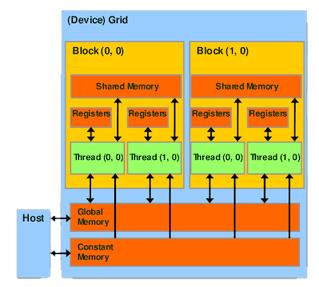
\includegraphics [trim = 0 0 0 0, clip, width=0.5\textwidth]{MEMORYY.png}
    %     %\caption{.}
    % \end{figure}
%*----------- notes
    \note[item]{Notes can help you to remember important information. Turn on the notes option.}
\end{frame}
%*----------- SLIDE -------------------------------------------------------------
\begin{frame}[t]{Thread}
    %\transboxin[duration=1,direction=30]
    \large
    Cada thread executa a mesma instrução mas em uma parte diferente dos dados\\
    SIMT - SINGLE INSTRUCTION MULTIPLE THREAD
%*----------- notes
    \note[item]{Notes can help you to remember important information. Turn on the notes option.}
\end{frame}
%-
%*----------- SLIDE -------------------------------------------------------------
\begin{frame}{Principais estudos da Bibliometria}
    % \begin{table}[ht!]
    %     \centering
    %         \caption{PERCENTUAL DE CONCLUSÃO POR EQUIPE}
    %         \begin{tabular}{|l|c|c|c|c|} \hline
    %             \textbf{EQUIPE}&\textbf{04/05}&\textbf{11/05}&\textbf{18/05}&\textbf{25/05}\\ \hline
    %             RAJA & 17\% &32\% & &  \\ \hline
    %             BORG & 0\% &41\% & &  \\ \hline
    %             TIMON-HM & 5\% &47\% & &  \\ \hline
    %         \end{tabular}
    % \end{table}

	\begin{table}[ht!]
		%\scalefont{0.7}
        \resizebox{0.9\textwidth}{!}{
		\begin{tabular}{|l|c|l|}
            \hline
            \multicolumn{1}{|c|}{\textbf{Leis e Princípios}} & \textbf{Foco de Estudo} & \multicolumn{1}{c|}{\textbf{Principais Aplicações}}                                                                         \\ \hline
            Lei de Bradford                                  & periódicos               & \begin{tabular}[c]{@{}l@{}}estimar o grau de relevância de periódicos\end{tabular}         \\ \hline
            Lei de Lotka                                     & autores                  & \begin{tabular}[c]{@{}l@{}}estimar o grau de relevância de autores\end{tabular}            \\ \hline
            Leis de Zipf                                     & palavras                 & \begin{tabular}[c]{@{}l@{}}indexação automática de artigos científicos\\ e tecnológicos\end{tabular}                        \\ \hline
            Fator de Impacto               & citações                 & \begin{tabular}[c]{@{}l@{}}estimar o grau de relevância de artigos, \\ cientistas e periódicos científicos\end{tabular} \\ \hline
            Acoplamento Bibliográfico                        & citações                 & \begin{tabular}[c]{@{}l@{}}estimar o grau de ligação de dois ou mais \\ artigos\end{tabular}                                \\ \hline
            Co-citação                                       & citações                 & \begin{tabular}[c]{@{}l@{}}estimar o grau de ligação de dois ou mais \\ artigos\end{tabular}                                \\ \hline
            Obsolescência da Literatura                      & citações                 & \begin{tabular}[c]{@{}l@{}}estimar o declínio da literatura de \\ determinada área do conhecimento\end{tabular}             \\ \hline
            Vida-média                                       & citações                 & \begin{tabular}[c]{@{}l@{}}estimar a vida-média de uma unidade da\\  literatura de dada área do conhecimento\end{tabular}   \\ \hline
		\end{tabular}
        }
	\end{table}

%*----------- notes
\note[item]{Notes can help you to remember important information. Turn on the notes option.}
\end{frame}
%-